\section{Background}
In this section, we first present an introduction to software-based 
side-channel attacks. Moreover, we analyze the root cause of many
software-based side-channels. We find many of them are caused by
two specific side-channel vulnerabilities, secret-dependent control-flow transfers and
secret-dependent memory accesses. Therefore, we will focus on identifying
and quantifying those leakages in the paper. After that, we 
discuss existing methods on side-channel detection and quantification.

\subsection{Software-based Side-channels}
Side-channels are information channels that can leak sensitive information 
unconsciously through different execution behaviors.  Fundamentally, those 
differences were caused by shared hardware
components (e.g., the CPU cache, the TLB and DRAM) in modern computer systems.
Depending on the layer causing side-channels, we can classify them 
into the following types of side-channel attacks.

For example, cached-based side-channels rely on the time differences 
between cache miss and cache hit. We introduce two common attack strategies,
namely Prime+Probe and Flush+Reload.
Prime+Probe targets a single cache set. The attacker preloads cache set with
its own data and wait until the victim execute the program.
If the victim accesses the cache set and evicts part of 
the data, the attacker will experience a slow measurement. If not, 
it will be fast. By knowing which cache set the target
program accesses, the attacker can infer locations of
the sensitive information. Flush+Reload targets a single cache line. 
It requires the attacker and the victim share the same memory address space.
During the ``flush'' stage, an attacker 
flushes the ``monitored memory'' from the cache. Then the attacker
waits for the victim to access the memory. In the next phase, the 
attacker reload the ``monitored memory''. By measuring the time difference, the
attacker can infer the sensitive information.

There are some other types of side-channels which target different hardware layers other than  
CPU cache.
For example, the controlled-channel attack~\cite{7163052},
where an attacker works in the kernel space, can infer sensitive data in the shielding systems by
observing the page fault sequences after restricting some code and
data pages. 

\begin{figure}
    \centering
    \subfloat[Mutual Information]
    {
        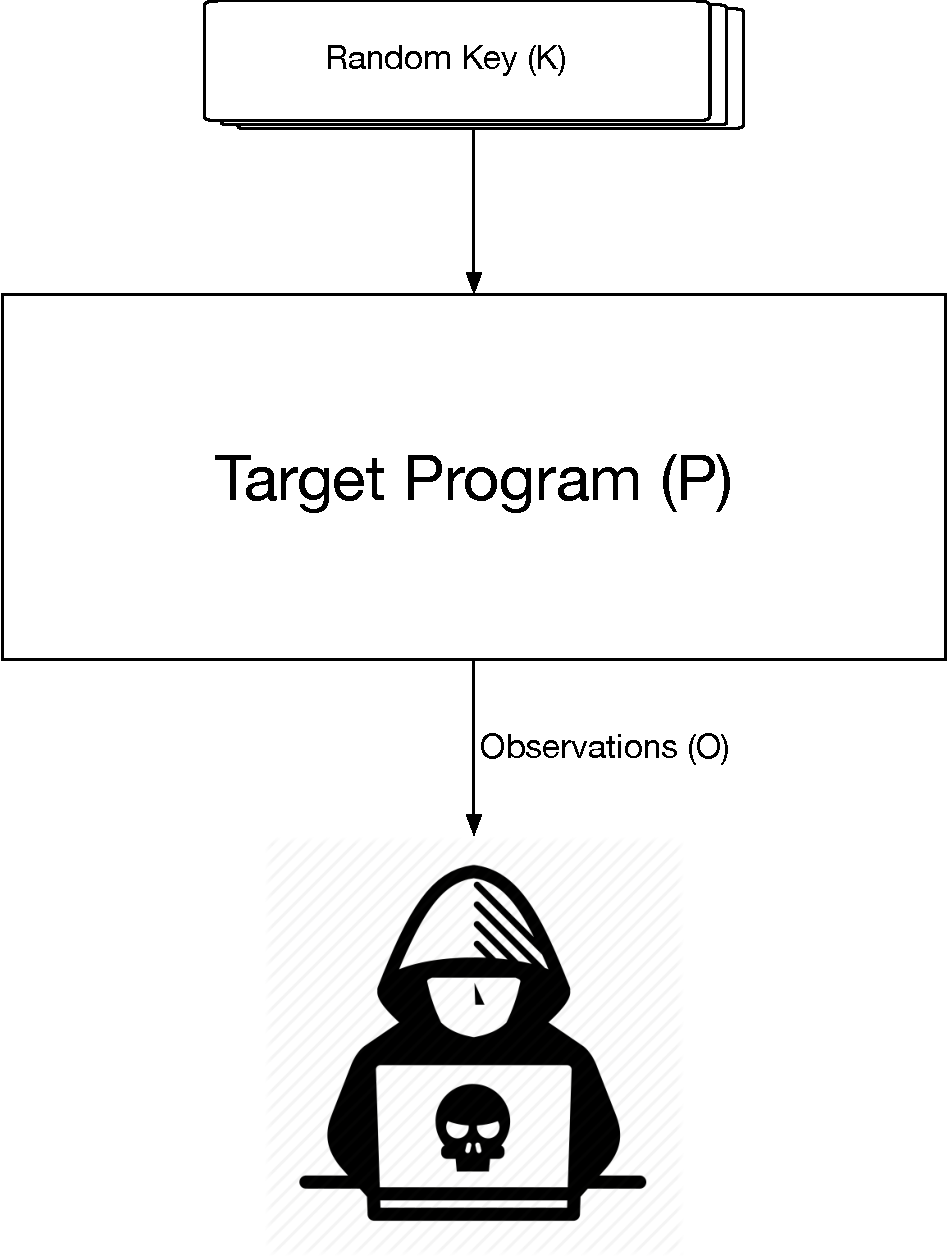
\includegraphics[width=.4\linewidth]{./figures/MI.pdf}
        \label{fig:1}
    }
    \subfloat[Real Attack]
    {
        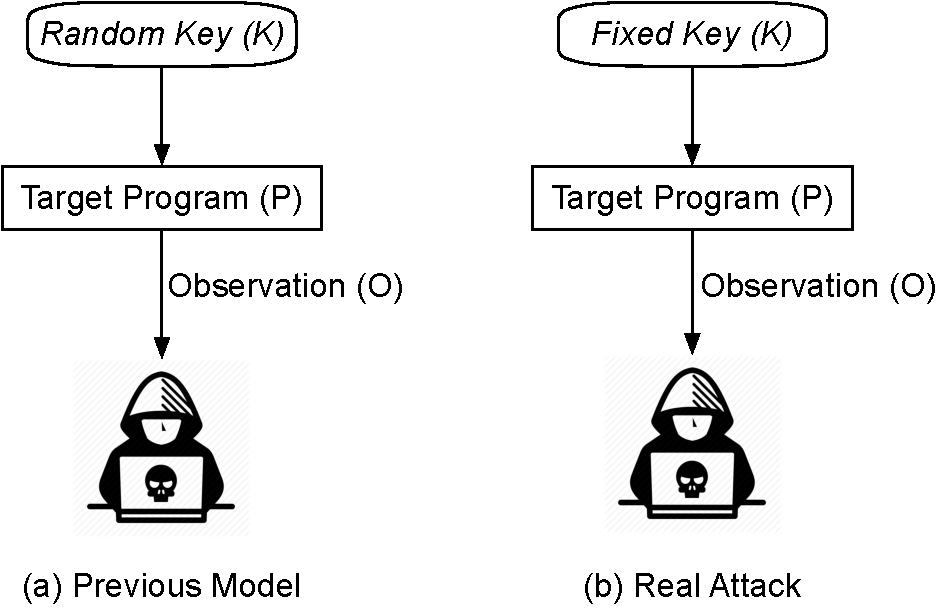
\includegraphics[width=.4\linewidth]{./figures/RA.pdf}
        \label{fig:2}
    }
    \caption{some caption here. \fixme{redraw the figure. i will give you the instruction.}}
    \end{figure}

The key intuition is that each side-channels above happens when the program accesses different 
memory addresses if the program has different sensitive inputs. More specifically, if 
a program show different patterns in control transfers or data accesses when the program 
processes different sensitive inputs, the program could possibly have side channels vulnerabilities. 
Different kinds of side-channels can be exploited to retrieve information
in various granularities. For example, many cache channels can observe cache accesses
at the level of a cache line. For most CPU, one cache line holds 64 bytes of data. So
the low 6 bits the address is irrelevant in causing those cached-based side-channels. 

%\lstinputlisting[language=c, 
%                 numbers=left,
%                 caption={Sample code shows secret-dependent memory access and 
%                          secret-dependent control-flow transfer.},
%                 captionpos=b,
%                 label={code:background},
%                 frame=single,
%                 basicstyle=\fontsize{7}{9}\selectfont\ttfamily]
%                 {sample_code/background.c}

%For example, the above code~\ref{code:background} show a simple encryption function that
%has the two kinds of side-channels. At line 11, depending on the value of a key,
%the code will access the different entry in the predefined table. At the
%line 13, the code will do a series of computation and determine if the code in the if
%branch is executed or not. Such vulnerabilities are called the memory-based 
%side-channles. We identify and quantify the leakage of the two kinds of vulnerabilities 
%in the paper.

\subsection{Information Leakage Quantification}

\fixme{Section (II.B), this subsection: Clarify mutual information, min-entropy, and maximal leakage. How many types? maybe use subsubsection}

Given an event $e$ which occurs with the probability $P(e)$, if the event $e$ happens, 
then we receive
\begin{displaymath}
    I = - \log_2P(e)
\end{displaymath}
bits of information by knowing the event $e$.
Consider a char variable $a$ in a C program, which has the size
of one byte (8 bits). It ranges from 0 -- 255.  Assume
 \textit{a} has the uniform distribution. If at one time we observe that $a$
equals $1$, the probability of this observation is $\frac{1}{256}$. So the information we get is 
$-\log(\frac{1}{256}) = 8$ bits, which is exactly the size of the char variable in the C program.

Some existing work on information leakage quantification is based on mutual information or 
min-entropy \cite{10.1007/978-3-642-00596-1_21}.
In these frameworks, the input sensitive
information $K$ is viewed as a random variable. Let $k_i$ be one of the possible
value of $K$. The Shannon entropy $H(K)$ is defined as
\begin{displaymath}
    H(K) = - \sum_{k_i {\in} K}P(k_i)\log_2P(k_i)
\end{displaymath}

The Shannon entropy can be used to quantify the initial uncertainty about the sensitive
information. Suppose a program with some
sensitive input $K$, an adversary has some observations ($O$) through some side channel.
In this work, the observations are referred as the secret-dependent control-flows and
secret-dependent data-access patterns. \fixme{See the comment above, we need to explain these
  patterns before this point.} The conditional entropy $H(K|O)$ is
\begin{displaymath}
    H(K|O) = - \sum_{o_j {\in} O} {P(o_j) \sum_{k_i {\in} K}{P(k_i|o_j)\log_2P(k_i|o_j)}}
\end{displaymath}
Intuitively, the conditional information marks the uncertainty about $K$ after the adversary
has gained some observations ($O$). 

Some previous work uses the mutual information $I(K; O)$ to quantify the leakage which is defined 
as follows:
\begin{displaymath}
    \mathit{Leakage} = I(K;O) = \sum_{k_i {\in} K}{\sum_{o_j {\in} O}{P(k_i, o_j)\log_2\frac{P(k_i, o_j)}{P(k_i)P(o_j)}}}
\end{displaymath}
where $P(k_i, o_i)$ is the joint discrete distribution of $K$ and $O$.
Alternatively, the mutual information can also be computed with the following equation:
\begin{displaymath}
    \mathit{Leakage} = I(K;O) = H(K) - H(K|O) = H(O) - H(O|K)
\end{displaymath}

For a deterministic program, once the input $K$ is fixed, the program will have the same
control-flow transfers and data-access patterns. As a result, $P(k_i, o_j)$ will always
equals to 1 or 0. So the conditional entropy $H(O|K)$ will equal to zero. So the leakage defined
by the mutual information can be simplified into:
\begin{displaymath}
\label{mutual:information}
    \mathit{Leakage} = I(K;O) = H(O)
\end{displaymath}
In other words, once we know the distribution of those memory-access patterns. We can 
calculate how much information is actually leaked.

Another common method is based on the maximal leakage~\cite{10.1007/978-3-642-00596-1_21,10.1007/978-3-642-31424-7_40,182946}.
The formal information theory can prove that the maximal leakage is the upper bound of the mutual 
information (Channel Capacity).

\begin{displaymath}
    \mathit{Leakage} = \log(C(O))
\end{displaymath}
Here $C(O)$ represents the number of different observations that an attacker can have. 

%% put this example in next section
%%\section{Running Example}

%Now we provide a concrete example to show how the two types of quantification definition works and show that
%how our method is different.

%\vspace{3pt}
%\textbf{Maximal Leakage.} 
%Depending on the value of key, the code can run four different branches which corrosponding to 
%four different observations. Therefore, by the maximal leakage definition, the leakage equals to 
%$\log4 = 2$ bits.

%\vspace{3pt}
%\textbf{Mutual Information.}
%If the key satisfies the uniform distribution, the probability of the code runs each branch
%can be computed with the following result.  

%\begin{table}[h]
%\centering
%\resizebox{\columnwidth}{!}{
%\begin{tabular}{|c|c|c|c|c|}
%\hline
%Branch & A     & B      & C      & D       \\ \hline
%Possibility      & 1/256 & 64/256 & 64/256 & 127/256 \\ \hline
%\end{tabular}
%}
%\caption{The distribution of observations}
%\end{table}

%Therefore, the leakage equals to 
%$\frac{1}{256}\log\frac{1}{256} + \frac{1}{4}\log\frac{1}{4}*2 + \frac{127}{256}\log\frac{127}{256} = 1.7$ bits.

%\vspace{3pt}
%\textbf{\tool.}
%\fixme{What is out result here? Need explain}
